\documentclass[a4paper,12pt,twoside,titlepage,openright]{book}
\usepackage[utf8]{inputenc}
\usepackage[T1]{fontenc}
\usepackage{microtype} % spezza le parole andando a capo solo se c'è DAVVERO bisogno
\usepackage{amsmath}
\usepackage{amssymb}
\usepackage{float}
\usepackage{graphicx}
\graphicspath{{Pictures}
             }
\usepackage{listings}
\usepackage{geometry}
\usepackage{todonotes}
\usepackage[autostyle=true,english=british]{csquotes}
\usepackage[backend=biber,
style=numeric,
sortlocale=de_DE,
natbib=true,
url=false, 
doi=true,
eprint=false]{biblatex}
\usepackage{latexsym}
\usepackage{bm}
\usepackage[format=plain,labelfont=bf]{caption}
\usepackage{subfig}
\usepackage[italian,english]{babel}
\usepackage[hidelinks]{hyperref} % aggiungere [hidelinks] per nascondere i quadranti rossi
\usepackage{cleveref}
\usepackage{afterpage} % permette di inserire pagine bianche
\usepackage{indentfirst} % indenta la prima riga di ogni nuova sezione
\usepackage{booktabs} % per le tabelle, permette di usare \toprule ecc
\usepackage{mathtools}
\usepackage{braket} % per fare le parentesi graffe degli insiemi
\usepackage{abraces}
\usepackage{multirow}
\usepackage{tablefootnote}
\usepackage[binding=5mm]{layaureo} 	% margini ottimizzati per l'A4; rilegatura di 5 mm
\usepackage[swapnames]{frontespizio}	% frontespizio 
%		% per includerlo nel documento bisogna:
%		% 1. compilare una prima volta main.tex;
%		% 2. compilare a parte main-frn.tex, generato dalla compilazione precedente;
%		% 3. compilare ancora main.tex.
%		% Non è necessario fare questi passaggi altre volte
%		% se il frontespizio non è più modificato.
\usepackage{changepage,calc}                 % centra il frontespizio
\usepackage{emptypage}		% pagine vuote senza testatina e piede di pagina
\usepackage{fancyhdr}		% testatine e piede personalizzati
\setlength{\headheight}{15pt}
\usepackage[super]{nth} % permette di usare \nth{1}, \nth{2}, \nth{3}, \nth{4} per 1st, 2nd ecc
\usepackage[footnote,		% descrizione acronimo fatta a piè di pagina
smaller,			% acronimo scritto con dimensione ridotta
]{acronym}		% acronimi
\usepackage{siunitx}
%\usepackage[symbols,nogroupskip,nonumberlist,automake]{glossaries-extra}

\newcommand{\sref}[1]{Section \ref{#1}}
\newcommand{\fref}[1]{Figure \ref{#1}}

%%%%%%%%%%%%%%%%%%%%%%%%%%%%%%%%%%%%%%%%%%%%%%%%%%%%%%%%%%%%%%%%%%%%%%%%%%%%%
\addbibresource{references/references.bib} %directory con le references
\AtBeginDocument{
	\renewcommand*{\mkbibnamefamily}[1]{\textsc{#1}}
}

% --------------------------------------------------------------------------- %
% !TEX encoding = UTF-8 Unicode
% !TEX TS-program = pdflatex
% !TEX root = main.tex
% !TEX spellcheck = it-IT
% --------------------------------------------------------------------------- %

\captionsetup{tableposition=top,
	figureposition=bottom,
	font=small,
	labelfont=bf}

\pagestyle{fancy}			% sostituisce \pagestyle{header} standard

\makeatletter 			% necessary for using \@chapapp
\renewcommand{\chaptermark}[1]{	% ridefinisce indicazione capitolo
  \markboth{\@chapapp\ \thechapter.\ #1}{}} % distinzione 'Capitolo' / 'Appendice'
\makeatother
%
\renewcommand{\sectionmark}[1]{	% ridefinisce indicazione sezione
	\markright{\thesection.\ #1}}
%
\fancyhf{}				% svuota testatine e piede
%
\fancyhead[LE,RO]{\bfseries\thepage}	% numero pagine in alto
%
\fancyhead[LO]{\bfseries\rightmark}	% info sezione nelle pag. dispari
%
\fancyhead[RE]{\bfseries\leftmark}	% info capitolo nelle pag.pari
%
\renewcommand{\headrulewidth}{0.4pt}	% spessore linea header
%
\renewcommand{\footrulewidth}{0pt}	% spessore linea footer (0pt=nascosta)
%
\fancypagestyle{plain}{				% ridefinizione stile inizio capitolo
		\fancyhead{}			% header vuoto
		\fancyfoot[C]{\bfseries\thepage}		% numeri in grassetto al centro
		\renewcommand{\headrulewidth}{0pt}	% no linea
		}
%
\newcommand{\scitel}[1]{$^[$\supercite{#1}$^]$}
\newcommand{\scitec}[1]{$^[$\supercite{#1}$^{],}$}

%\makeglossaries

%\glsxtrnewsymbol[description={angle of attack}]{alpha}{\ensuremath{\alpha}}
%\glsxtrnewsymbol[description={2-D lift coefficinet}]{Cl}{\ensuremath{C_l}}
%\glsxtrnewsymbol[description={vortex generator chord}]{cvg}{\ensuremath{c_{vg}}}
%\glsxtrnewsymbol[description={target profile chord}]{ctp}{\ensuremath{c_{tp}}}
%\glsxtrnewsymbol[description={vortex core diameter}]{dcore}{\ensuremath{d_{core}}}
%\glsxtrnewsymbol[description={vorticity vector}]{omega}{\ensuremath{\bm{\omega}}}
%\glsxtrnewsymbol[description={frequency}]{freq}{\ensuremath{\omega}}
%\glsxtrnewsymbol[description={lift for unit span}]{L2D}{\ensuremath{L_{2D}}}
%\glsxtrnewsymbol[description={air kinematic viscosity}]{nu}{\ensuremath{\nu}}
%\glsxtrnewsymbol[description={air density}]{rho}{\ensuremath{\rho}}
%\glsxtrnewsymbol[description={radial distance from the vortex center}]{r}{\ensuremath{r}}
%\glsxtrnewsymbol[description={velocity vector}]{u}{\ensuremath{\bm{u}}}
%\glsxtrnewsymbol[description={circulation}]{Gamma}{\ensuremath{\Gamma}}
%\glsxtrnewsymbol[description={vortex generation circulation}]{Gammavg}{\ensuremath{\Gamma_{vg}}}
%\glsxtrnewsymbol[description={vortex circulation}]{Gammavtx}{\ensuremath{\Gamma_{vtx}}}
%\glsxtrnewsymbol[description={advancing ratio}]{mu}{\ensuremath{\mu}}
%\glsxtrnewsymbol[description={non dimensional frequency}]{k}{\ensuremath{k}}
%\glsxtrnewsymbol[description={actuation time}]{Deltat}{\ensuremath{\Delta t}}
%\glsxtrnewsymbol[description={vortex generator Reynolds number}]{Revg}{\ensuremath{Re_{vg}}}
%\glsxtrnewsymbol[description={target profile Reynolds number}]{Retp}{\ensuremath{Re_{tp}}}
%\glsxtrnewsymbol[description={Wind tunnel freestream velocity}]{Vinf}{\ensuremath{V_\infty}}
%\glsxtrnewsymbol[description={Slope of the Lift coefficient curve}]{Clalpha}{\ensuremath{C_{l/\alpha}}}

\begin{document}
	
\frontmatter
% Inizio del Frontespizio

\thispagestyle{empty}
\enlargethispage{60mm}
\begin{center}
\Large{\textsc{Politecnico di Milano}}\\
%\vspace{5mm}
\large{Facolt\`a di Ingegneria}\\
%\vspace{5mm}
\large{Corso di laurea in Ingegneria Aeronautica}\\
\large{Dipartimento di Scienze e Tecnologie Aerospaziali}\\
\vspace{7mm}
\begin{figure}[h]
\begin{center}
%\includegraphics[scale=0.15]{img/logo.png}
\end{center}
\end{figure}
\vspace{2mm}

% titolo della tesi
\begin{LARGE}
LOREM IPSUM
\end{LARGE}
\vspace{25mm}

% relatore
\begin{flushleft}
\begin{tabular}{l l }
Relatore:    & Prof. Giuseppe Gibertini\\
%Correlatore: & Ing. Nome COGNOME\\
\end{tabular}
\end{flushleft}
\vspace{25mm}

% autore/autori
\begin{flushright}
\begin{tabular}{l l }
Tesi di Laurea di: & \\
Matteo Bramati & Matr. 898950
\end{tabular}
\end{flushright}
\vspace{43mm}
{\large{\bf Anno Accademico 2018-2019}}
\end{center}
\cleardoublepage
%inserire tutto ciò che è personale
%\input{secretato}
\cleardoublepage
\tableofcontents
%\listoffigures
%\listoftables
		
\cleardoublepage

\mainmatter
%\input{intro}
%\chapter{SU2}
Introduction to SU2

\section{Governing Equations}
Navier-Stokes

\subsection{Incompressible Navier - Stokes}

SU2 solves the incompressible Navier-Stokes equations in a general form allowing for variable density due to heat transfer through the low-Mach approximation (or incompressible ideal gas formulation). The equations can be expressed in differential form as 
\begin{equation}
	
\end{equation}
%\input{PoliMIce}

%% Indice Provvisorio: Inserire ogni capitolo in un documento a parte.
\chapter{Introduction}
\label{sec: intro}

	\section{The \textit{Snow Problem} for in-flight ice accretion}
	\label{sec: SnowProblem}
		Why studying the snow is relevant for in-flight ice accretion. What PoliMIce (PoliDrop) needs from this study: $ c_D(Re, param) $ formula and a rule to choose the parameters.
		
	\section{Non-spherical particles}
		Introduction to non-spherical particles models: types of models and experiments available (relative to a generic non-spherical particles) and the principal shape factors.
		
		\textbf{Models and Experiments examples}\\
		Explanation of figures like \ref{fig: cube} and \ref{fig: cylinder}.
		
		\begin{figure}[]
			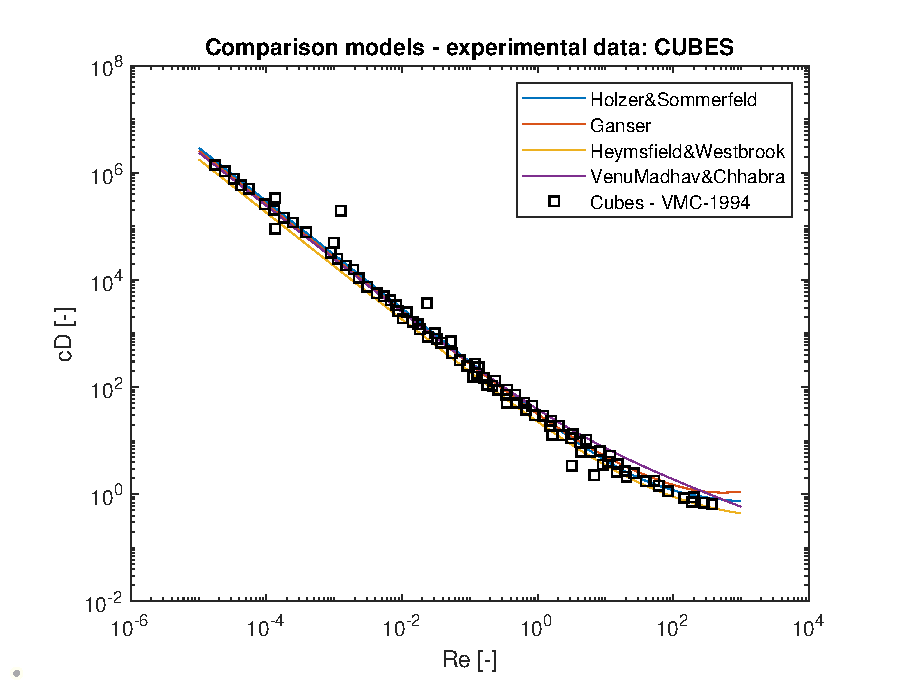
\includegraphics{cube_cD.eps}
			\caption{}
			\label{fig: cube}
		\end{figure}
		\begin{figure}[]
			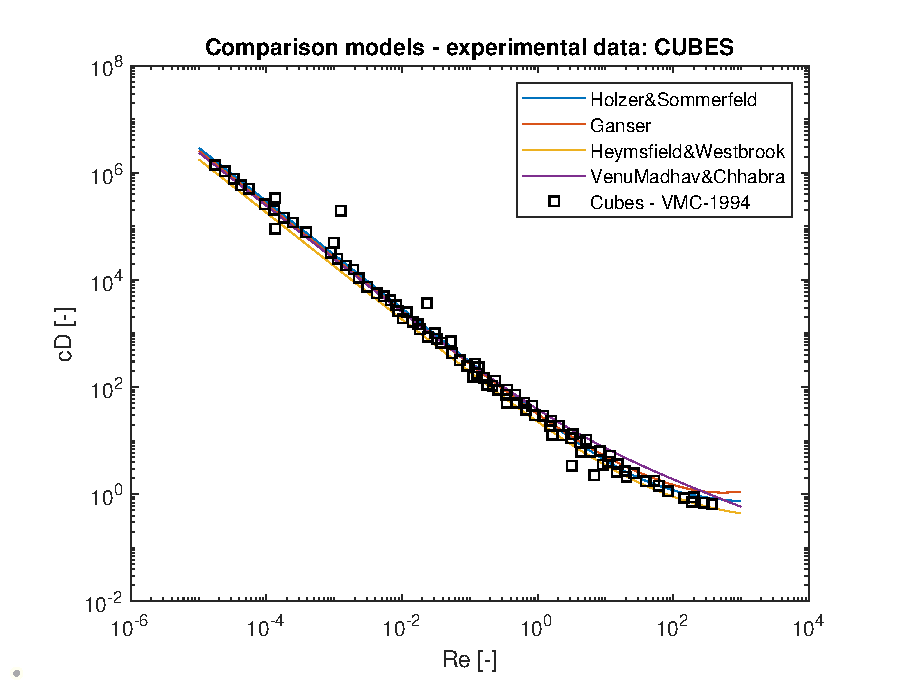
\includegraphics{cube_cD.eps}
			\caption{}
			\label{fig: cylinder}
		\end{figure}
	
	\section{Snow experiments}
		Introduction to available snow experiments. For aerodynamic purposes the most relevant type of measure is the ground experiment conducted with some kind of disdrometer. It gives a measure the particle dimension (often its mean diameter) and a measure of its terminal velocity.
		
	\section{Blowing vs Falling regime}
		Problem with the difference between the regime of the simulations and the regime of the experiments. Our assumption: the model we chose is able to transfer the information about the shape of the particle from the falling to the blowing regime.

		
	\section{Problem Formulation}
		Goal of the thesis: The question proposed in \sref{sec: SnowProblem} will be answered by:
		\begin{enumerate}
			\item Find a suitable model for the description of the snow $ c_D $
			\item Use that model to infer the statistical distribution of the shape parameters of a given \textit{cloud} in the \textit{falling regime}
			\item Transfer this information to the \textit{blowing regime} by implementing the same model with the same parameter distribution in PoliDrop
		\end{enumerate}	

	\section{Structure of the thesis}
		Chapter description
		
		
\chapter{Choice of the Model}
	\section{Chhabra review: Ganser}
		The models must provide information on 2 main aspect: \textit{shape} of the particle (sphericity) and \textit{orientation} of the particle. (Chhabra)
		Description of the Ganser model (The best up to 1993).
		\\
		
		Description of the more recent models (2004? and 2008)
				
	\section{Heymsfield and Westbrook - (2004)}
		Description of the model ans why it doesn't work.
		(Do I need to talk about this model?)
		
	\section{Holzer and Sommerfeld - (2008)}
		Description of the model and it's simplified form. Comparison with Ganser: sensitivity study on the parameters of both models and why H\&S better suits the experimental curves of snow
		(+ "cite" the ICE GENESIS results proving that this model is the better one)

	
\chapter{Description of the Data Set}
	Type of information needed for the parameter estimation ($ d_v $ (some measure of the diameter), $ v_t $ (terminal velocity), $ \sigma $ (measurement error)).
	
	Brief description of the available experimental campaigns (Brandes + other 2 references) and their limitations.
	
	\section{Brandes Experimental campaign}
		Description of the Brandes results and impossibility to use the raw data
		
	\section{Data Set generation}
		Generation of an artificial data set starting from the relations discovered by Brandes. The dependency on the diameter distribution is not taken into account as it can be retrieved a posteriori.


\chapter{Parameter Estimation}
	\section{Problem Formulation}
		Variables, unknown, data declaration.

	\section{Bayes Theorem}
		Theoretical background on Data Analysis using the Bayes approach. Choice of the prior and the likelihood to find the single, best parameter that explains a certain data set.
		
	\section{Gaussian Mixture Model}
		Need of a multi-modal distribution of the parameter: in a cloud more that one type of shape can be present. Modification of the Likelihood function using GMMs.
		
	\section{General scheme}
		General scheme of the program: Iteratively increase the number of mode allowed up to a certain convergence criterion (Da vedere con Giulio)
	
	
\chapter{Numerical Implementation}
	\section{Terminal Velocity calculation}
		Equation for the terminal velocity of a particle: how to calculate every term starting from the diameter and the shape parameters
		
	\section{Maximization of the Posterior/Likelihood}
		Calculation of a single posterior element
		\begin{itemize}
			\item brute force algorithm
			\item optimization (Genetic Algorithm)
			\item Markov-chain method (?)
		\end{itemize}
	
	\section{Code Validation}
		Validation with totally artificial data set
		\begin{itemize}
			\item 1 parameter (\fref{val: 1paramData}, \ref{val: 1param1}, \ref{val: 1param2}, \ref{val: 1param3})
			\item 2 parameters (\fref{val: 2paramData}, \ref{val: 2param1}, \ref{val: 2param2})
		\end{itemize}
	
		\begin{figure}
			\centering
			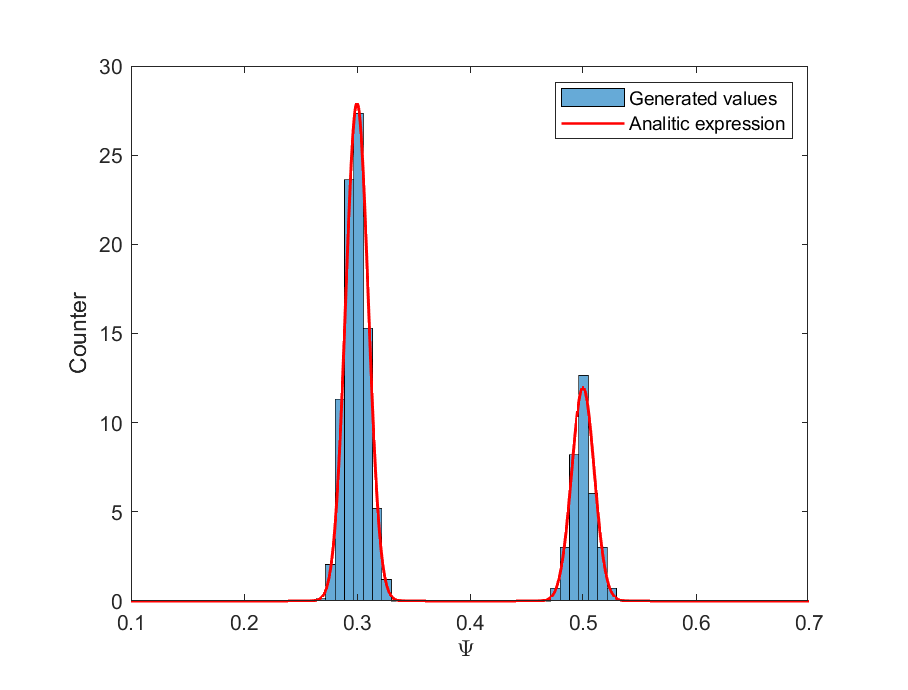
\includegraphics{validation/1paramData.eps}
			\caption{}
			\label{val: 1paramData}
		\end{figure}
		\begin{figure}
			\centering
			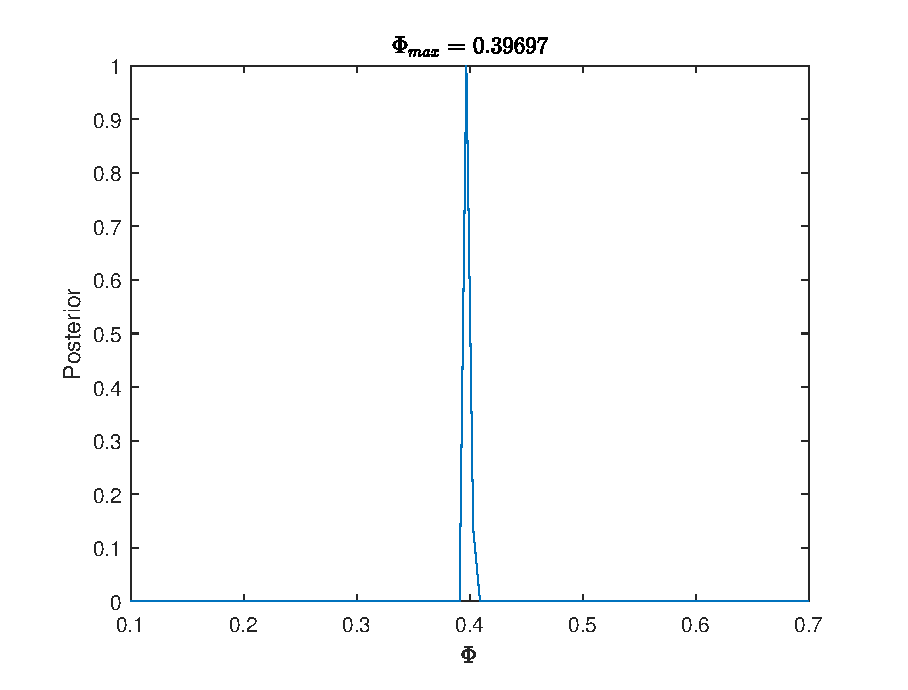
\includegraphics{validation/1param1.eps}
			\caption{}
			\label{val: 1param1}
		\end{figure}
		\begin{figure}
			\centering
			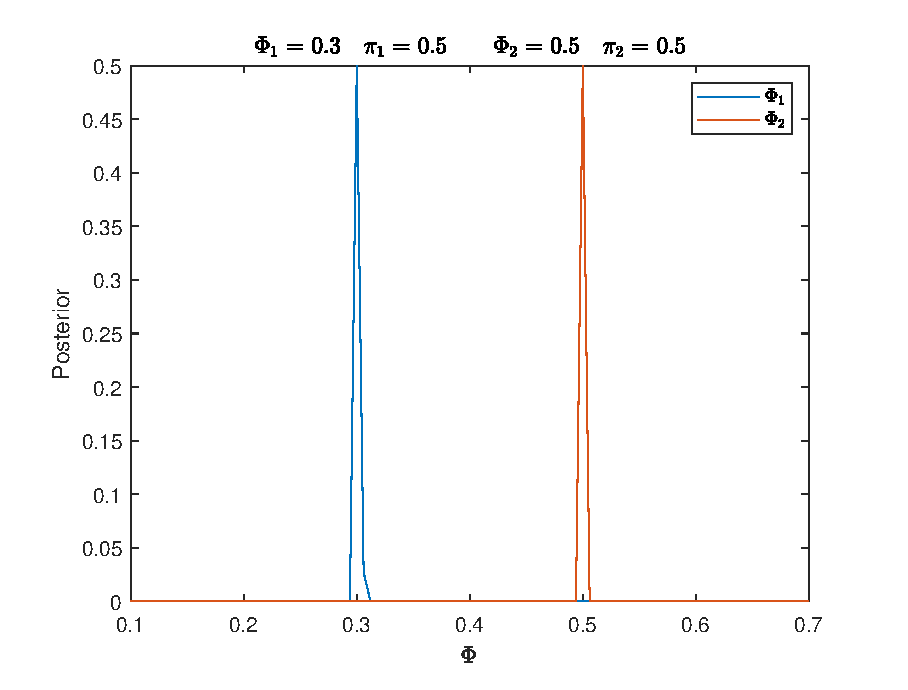
\includegraphics{validation/1param2.eps}
			\caption{}
			\label{val: 1param2}
		\end{figure}
		\begin{figure}
			\centering
			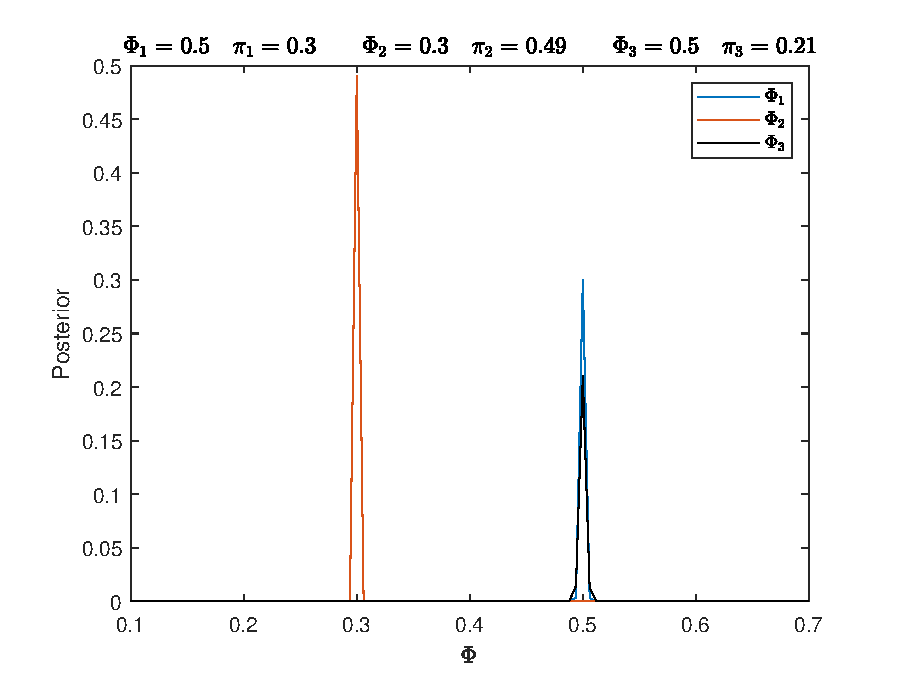
\includegraphics{validation/1param3.eps}
			\caption{}
			\label{val: 1param3}
		\end{figure}

		\begin{figure}
			\centering
			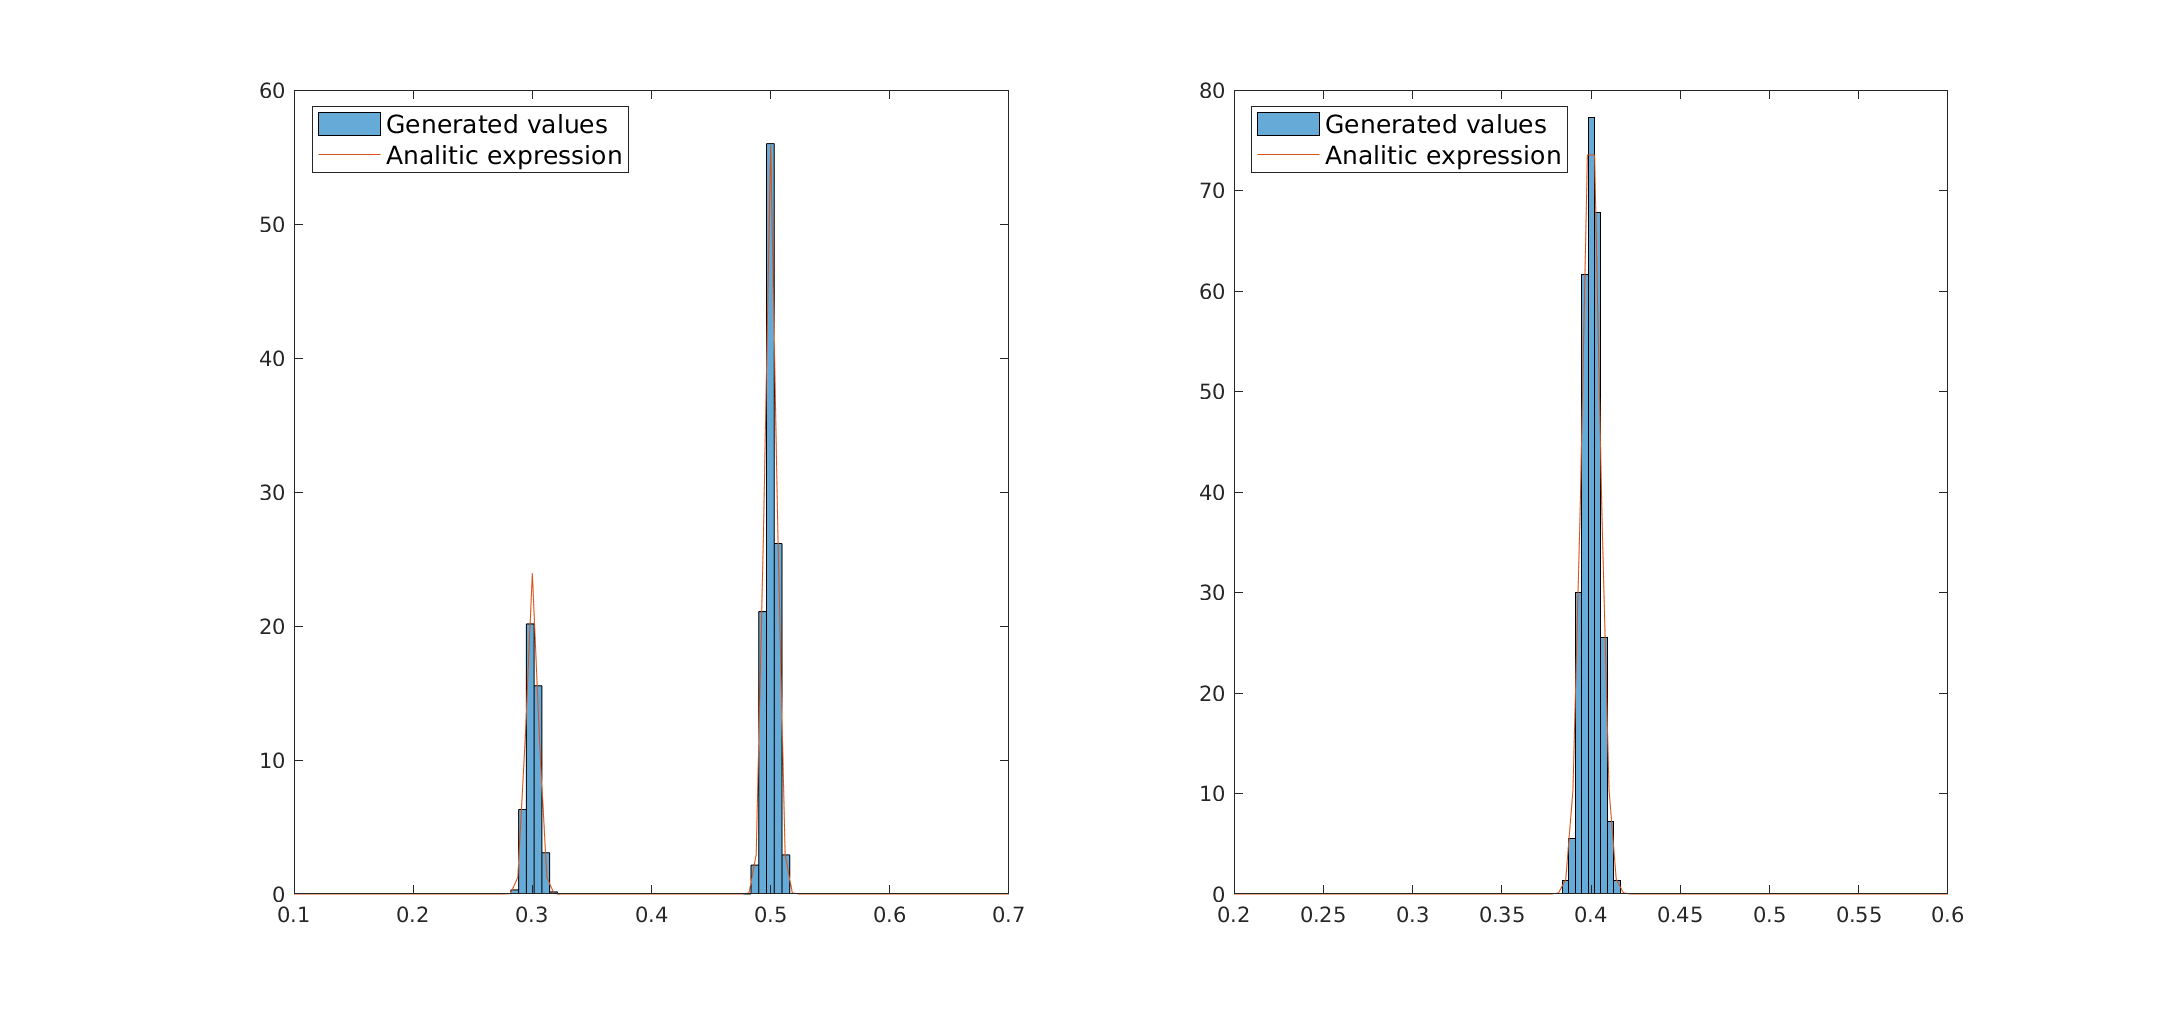
\includegraphics[width=\linewidth]{validation/2paramData.eps}
			\caption{}
			\label{val: 2paramData}
		\end{figure}
		\begin{figure}
			\centering
			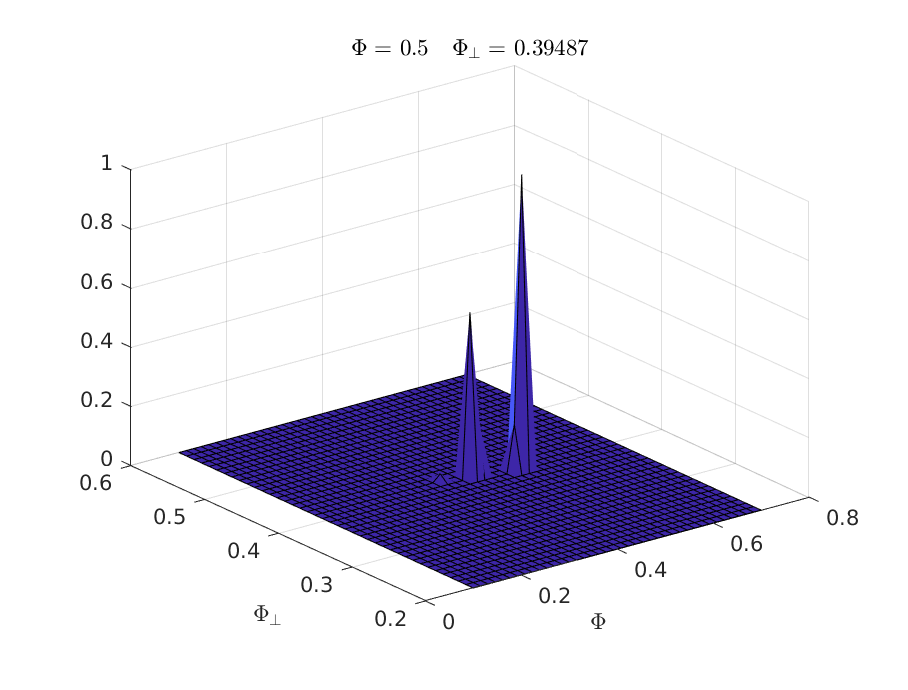
\includegraphics[width=\linewidth]{validation/2param1.eps}
			\caption{}
			\label{val: 2param1}
		\end{figure}
		\begin{figure}
			\centering
			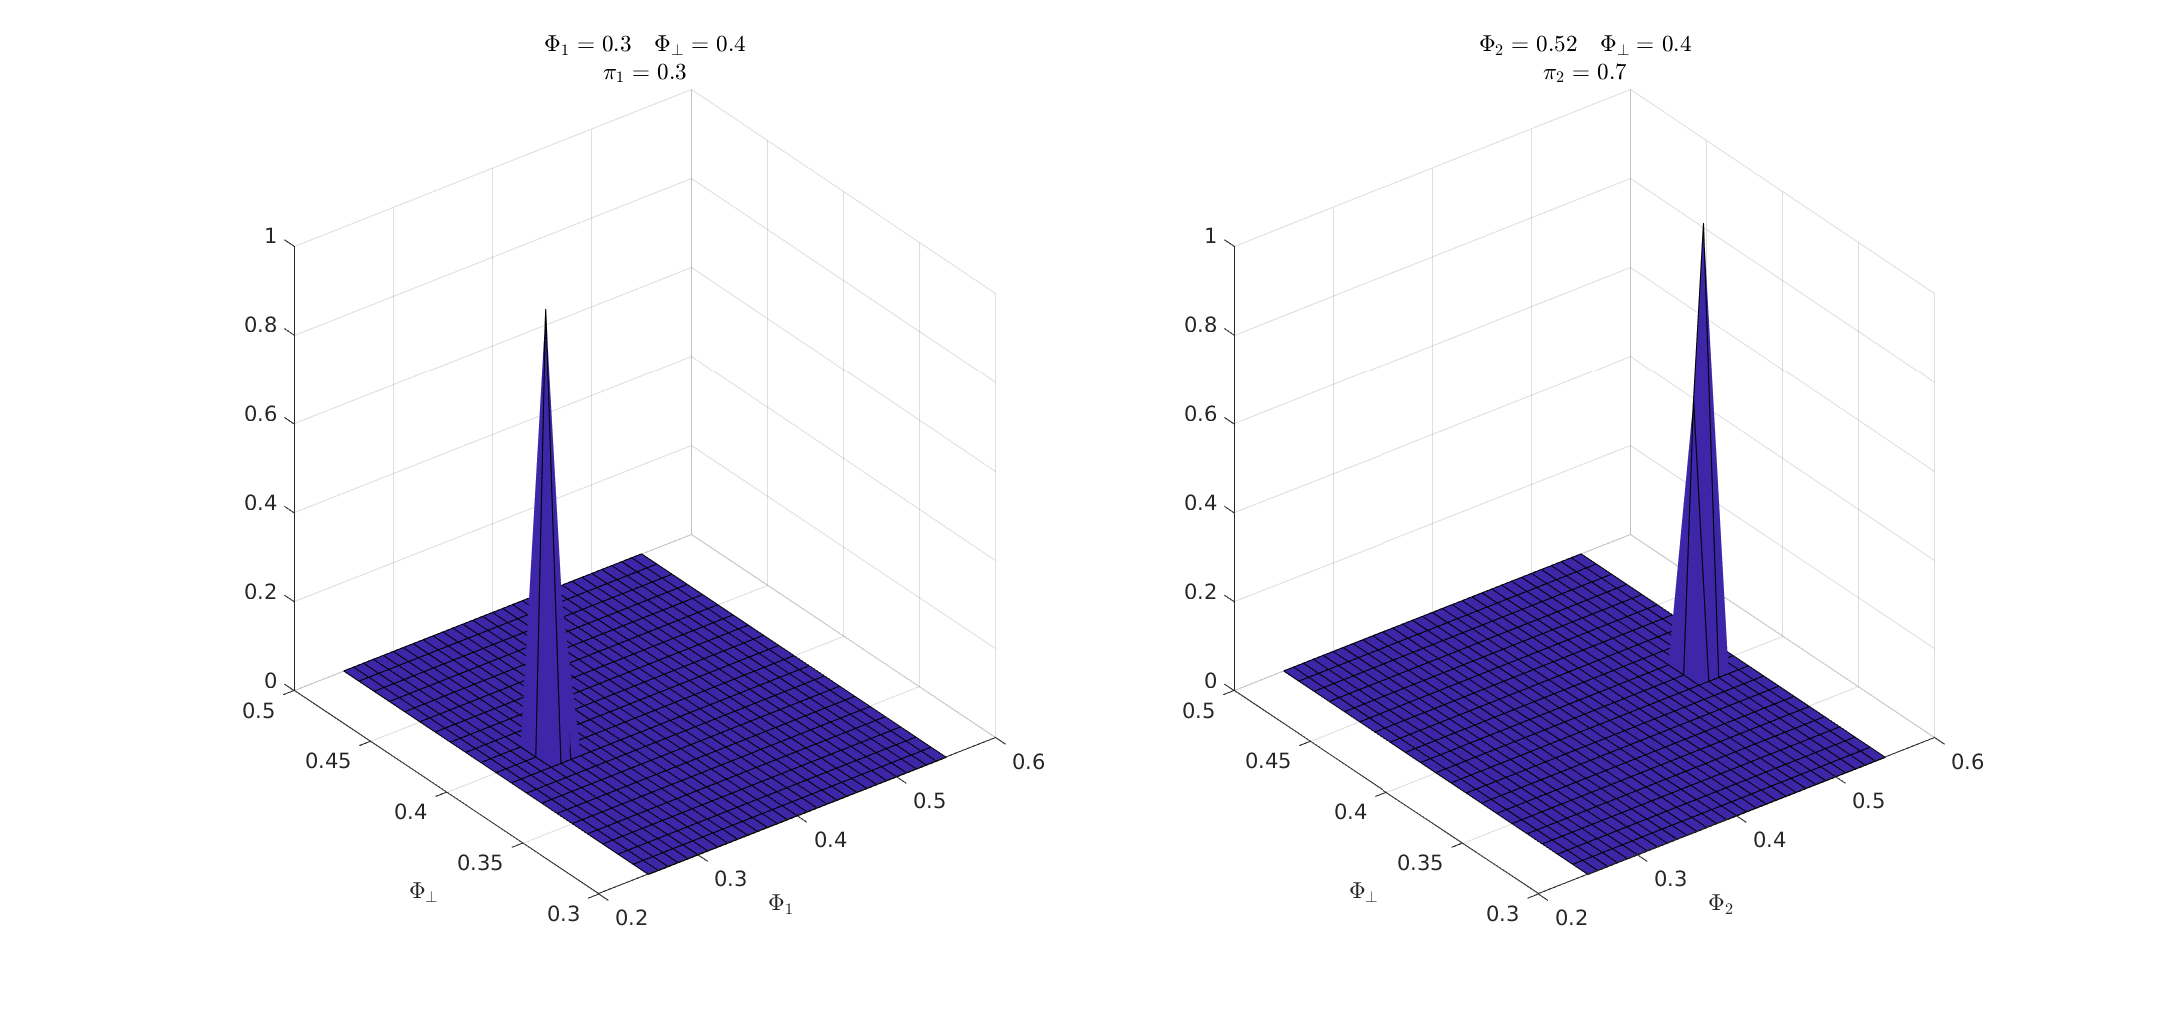
\includegraphics[width=\linewidth]{validation/2param2.eps}
			\caption{}
			\label{val: 2param2}
		\end{figure}

	\section{Results}
		Application to the Brandes data set: 
		\begin{itemize}
			\item Example for 1 diameter interval
			\item Shape parameters - diameter distribution (Work in progress)
		\end{itemize}
		
	
\chapter{Integration to PoliMIce (To Do)}
	Implementation of the chosen formula for the $ c_D $ in PoliDrop
	
	\section{Cloud generation}
		Some rules to generate the cloud by PoliDrop
		
	\section{Results}
		\subsection{Let it snow!}
			Falling snow test case (Check the terminal velocity distribution for validation?)
			
		\subsection{Blowing snow example}
			Blowing snow test case: ice accretion on a profile?


\chapter{Conclusions and Future developments}

	
\printbibliography[heading=bibintoc]
\end{document}